% Options for packages loaded elsewhere
\PassOptionsToPackage{unicode}{hyperref}
\PassOptionsToPackage{hyphens}{url}
\PassOptionsToPackage{dvipsnames,svgnames,x11names}{xcolor}
%
\documentclass[
  ignorenonframetext,
]{beamer}
\usepackage{pgfpages}
\setbeamertemplate{caption}[numbered]
\setbeamertemplate{caption label separator}{: }
\setbeamercolor{caption name}{fg=normal text.fg}
\beamertemplatenavigationsymbolsempty
% Prevent slide breaks in the middle of a paragraph
\widowpenalties 1 10000
\raggedbottom
\setbeamertemplate{part page}{
  \centering
  \begin{beamercolorbox}[sep=16pt,center]{part title}
    \usebeamerfont{part title}\insertpart\par
  \end{beamercolorbox}
}
\setbeamertemplate{section page}{
  \centering
  \begin{beamercolorbox}[sep=12pt,center]{part title}
    \usebeamerfont{section title}\insertsection\par
  \end{beamercolorbox}
}
\setbeamertemplate{subsection page}{
  \centering
  \begin{beamercolorbox}[sep=8pt,center]{part title}
    \usebeamerfont{subsection title}\insertsubsection\par
  \end{beamercolorbox}
}
\AtBeginPart{
  \frame{\partpage}
}
\AtBeginSection{
  \ifbibliography
  \else
    \frame{\sectionpage}
  \fi
}
\AtBeginSubsection{
  \frame{\subsectionpage}
}
\usepackage{amsmath,amssymb}
\usepackage{lmodern}
\usepackage{iftex}
\ifPDFTeX
  \usepackage[T1]{fontenc}
  \usepackage[utf8]{inputenc}
  \usepackage{textcomp} % provide euro and other symbols
\else % if luatex or xetex
  \usepackage{unicode-math}
  \defaultfontfeatures{Scale=MatchLowercase}
  \defaultfontfeatures[\rmfamily]{Ligatures=TeX,Scale=1}
\fi
% Use upquote if available, for straight quotes in verbatim environments
\IfFileExists{upquote.sty}{\usepackage{upquote}}{}
\IfFileExists{microtype.sty}{% use microtype if available
  \usepackage[]{microtype}
  \UseMicrotypeSet[protrusion]{basicmath} % disable protrusion for tt fonts
}{}
\makeatletter
\@ifundefined{KOMAClassName}{% if non-KOMA class
  \IfFileExists{parskip.sty}{%
    \usepackage{parskip}
  }{% else
    \setlength{\parindent}{0pt}
    \setlength{\parskip}{6pt plus 2pt minus 1pt}}
}{% if KOMA class
  \KOMAoptions{parskip=half}}
\makeatother
\usepackage{xcolor}
\newif\ifbibliography
\usepackage{color}
\usepackage{fancyvrb}
\newcommand{\VerbBar}{|}
\newcommand{\VERB}{\Verb[commandchars=\\\{\}]}
\DefineVerbatimEnvironment{Highlighting}{Verbatim}{commandchars=\\\{\}}
% Add ',fontsize=\small' for more characters per line
\usepackage{framed}
\definecolor{shadecolor}{RGB}{248,248,248}
\newenvironment{Shaded}{\begin{snugshade}}{\end{snugshade}}
\newcommand{\AlertTok}[1]{\textcolor[rgb]{0.94,0.16,0.16}{#1}}
\newcommand{\AnnotationTok}[1]{\textcolor[rgb]{0.56,0.35,0.01}{\textbf{\textit{#1}}}}
\newcommand{\AttributeTok}[1]{\textcolor[rgb]{0.77,0.63,0.00}{#1}}
\newcommand{\BaseNTok}[1]{\textcolor[rgb]{0.00,0.00,0.81}{#1}}
\newcommand{\BuiltInTok}[1]{#1}
\newcommand{\CharTok}[1]{\textcolor[rgb]{0.31,0.60,0.02}{#1}}
\newcommand{\CommentTok}[1]{\textcolor[rgb]{0.56,0.35,0.01}{\textit{#1}}}
\newcommand{\CommentVarTok}[1]{\textcolor[rgb]{0.56,0.35,0.01}{\textbf{\textit{#1}}}}
\newcommand{\ConstantTok}[1]{\textcolor[rgb]{0.00,0.00,0.00}{#1}}
\newcommand{\ControlFlowTok}[1]{\textcolor[rgb]{0.13,0.29,0.53}{\textbf{#1}}}
\newcommand{\DataTypeTok}[1]{\textcolor[rgb]{0.13,0.29,0.53}{#1}}
\newcommand{\DecValTok}[1]{\textcolor[rgb]{0.00,0.00,0.81}{#1}}
\newcommand{\DocumentationTok}[1]{\textcolor[rgb]{0.56,0.35,0.01}{\textbf{\textit{#1}}}}
\newcommand{\ErrorTok}[1]{\textcolor[rgb]{0.64,0.00,0.00}{\textbf{#1}}}
\newcommand{\ExtensionTok}[1]{#1}
\newcommand{\FloatTok}[1]{\textcolor[rgb]{0.00,0.00,0.81}{#1}}
\newcommand{\FunctionTok}[1]{\textcolor[rgb]{0.00,0.00,0.00}{#1}}
\newcommand{\ImportTok}[1]{#1}
\newcommand{\InformationTok}[1]{\textcolor[rgb]{0.56,0.35,0.01}{\textbf{\textit{#1}}}}
\newcommand{\KeywordTok}[1]{\textcolor[rgb]{0.13,0.29,0.53}{\textbf{#1}}}
\newcommand{\NormalTok}[1]{#1}
\newcommand{\OperatorTok}[1]{\textcolor[rgb]{0.81,0.36,0.00}{\textbf{#1}}}
\newcommand{\OtherTok}[1]{\textcolor[rgb]{0.56,0.35,0.01}{#1}}
\newcommand{\PreprocessorTok}[1]{\textcolor[rgb]{0.56,0.35,0.01}{\textit{#1}}}
\newcommand{\RegionMarkerTok}[1]{#1}
\newcommand{\SpecialCharTok}[1]{\textcolor[rgb]{0.00,0.00,0.00}{#1}}
\newcommand{\SpecialStringTok}[1]{\textcolor[rgb]{0.31,0.60,0.02}{#1}}
\newcommand{\StringTok}[1]{\textcolor[rgb]{0.31,0.60,0.02}{#1}}
\newcommand{\VariableTok}[1]{\textcolor[rgb]{0.00,0.00,0.00}{#1}}
\newcommand{\VerbatimStringTok}[1]{\textcolor[rgb]{0.31,0.60,0.02}{#1}}
\newcommand{\WarningTok}[1]{\textcolor[rgb]{0.56,0.35,0.01}{\textbf{\textit{#1}}}}
\usepackage{graphicx}
\makeatletter
\def\maxwidth{\ifdim\Gin@nat@width>\linewidth\linewidth\else\Gin@nat@width\fi}
\def\maxheight{\ifdim\Gin@nat@height>\textheight\textheight\else\Gin@nat@height\fi}
\makeatother
% Scale images if necessary, so that they will not overflow the page
% margins by default, and it is still possible to overwrite the defaults
% using explicit options in \includegraphics[width, height, ...]{}
\setkeys{Gin}{width=\maxwidth,height=\maxheight,keepaspectratio}
% Set default figure placement to htbp
\makeatletter
\def\fps@figure{htbp}
\makeatother
\setlength{\emergencystretch}{3em} % prevent overfull lines
\providecommand{\tightlist}{%
  \setlength{\itemsep}{0pt}\setlength{\parskip}{0pt}}
\setcounter{secnumdepth}{-\maxdimen} % remove section numbering
\usepackage{graphicx}
\usepackage{bm}
\usepackage{array}
\usepackage{amsmath}
\usepackage{amsthm}
\usepackage{amsfonts}
\usepackage{amssymb}
\usepackage{tikz-cd}
\usepackage{url}
\definecolor{foreground}{RGB}{255,255,255}
\definecolor{background}{RGB}{34,28,54}
\definecolor{title}{RGB}{105,165,255}
\definecolor{gray}{RGB}{175,175,175}
\definecolor{lightgray}{RGB}{225,225,225}
\definecolor{subtitle}{RGB}{232,234,255}
\definecolor{hilight}{RGB}{112,224,255}
\definecolor{vhilight}{RGB}{255,111,207}
\setbeamertemplate{footline}[page number]
\ifLuaTeX
  \usepackage{selnolig}  % disable illegal ligatures
\fi
\IfFileExists{bookmark.sty}{\usepackage{bookmark}}{\usepackage{hyperref}}
\IfFileExists{xurl.sty}{\usepackage{xurl}}{} % add URL line breaks if available
\urlstyle{same} % disable monospaced font for URLs
\hypersetup{
  pdftitle={STAT 528 - Advanced Regression Analysis II},
  pdfauthor={Data Separation (part II)},
  colorlinks=true,
  linkcolor={Maroon},
  filecolor={Maroon},
  citecolor={Blue},
  urlcolor={blue},
  pdfcreator={LaTeX via pandoc}}

\title{STAT 528 - Advanced Regression Analysis II}
\author{Data Separation (part II)}
\date{}
\institute{Daniel J. Eck\\
Department of Statistics\\
University of Illinois}

\begin{document}
\frame{\titlepage}

\begin{frame}
\newcommand{\R}{\mathbb{R}}
\newcommand{\Prob}{\mathbb{P}}
\newcommand{\Proj}{\textbf{P}}
\newcommand{\Hcal}{\mathcal{H}}
\newcommand{\rootn}{\sqrt{n}}
\newcommand{\p}{\mathbf{p}}
\newcommand{\E}{\text{E}}
\newcommand{\Var}{\text{Var}}
\newcommand{\Cov}{\text{Cov}}
\newcommand{\mubf}{\bm{\mu}}
\newcommand{\logit}{\text{logit}}

\newtheorem{cor}{Corollary}
\newtheorem{lem}{Lemma}
\newtheorem{thm}{Theorem}
\newtheorem{defn}{Definition}
\newtheorem{prop}{Proposition}
\end{frame}

\begin{frame}{Today's Learning Objectives}
\protect\hypertarget{todays-learning-objectives}{}
\begin{itemize}
\tightlist
\item
  data separation introduction
\item
  statistical inference when separation exists
\end{itemize}

\vspace{12pt}

This slide deck will only contain data analyses and computational tools.
\end{frame}

\begin{frame}[fragile]{}
\protect\hypertarget{section}{}
Recall our 8 point data set which is taken from Section 6.5.1 in
Agresti.

\vspace{12pt}
\tiny

\begin{Shaded}
\begin{Highlighting}[]
\NormalTok{x }\OtherTok{\textless{}{-}}\NormalTok{ (}\DecValTok{1}\SpecialCharTok{:}\DecValTok{9} \SpecialCharTok{*} \DecValTok{10}\NormalTok{)[}\SpecialCharTok{{-}}\DecValTok{5}\NormalTok{]}
\NormalTok{y }\OtherTok{\textless{}{-}} \FunctionTok{c}\NormalTok{(}\DecValTok{0}\NormalTok{,}\DecValTok{0}\NormalTok{,}\DecValTok{0}\NormalTok{,}\DecValTok{0}\NormalTok{,}\DecValTok{1}\NormalTok{,}\DecValTok{1}\NormalTok{,}\DecValTok{1}\NormalTok{,}\DecValTok{1}\NormalTok{)}
\FunctionTok{plot}\NormalTok{(x, y, }\AttributeTok{pch =} \DecValTok{19}\NormalTok{)}
\end{Highlighting}
\end{Shaded}

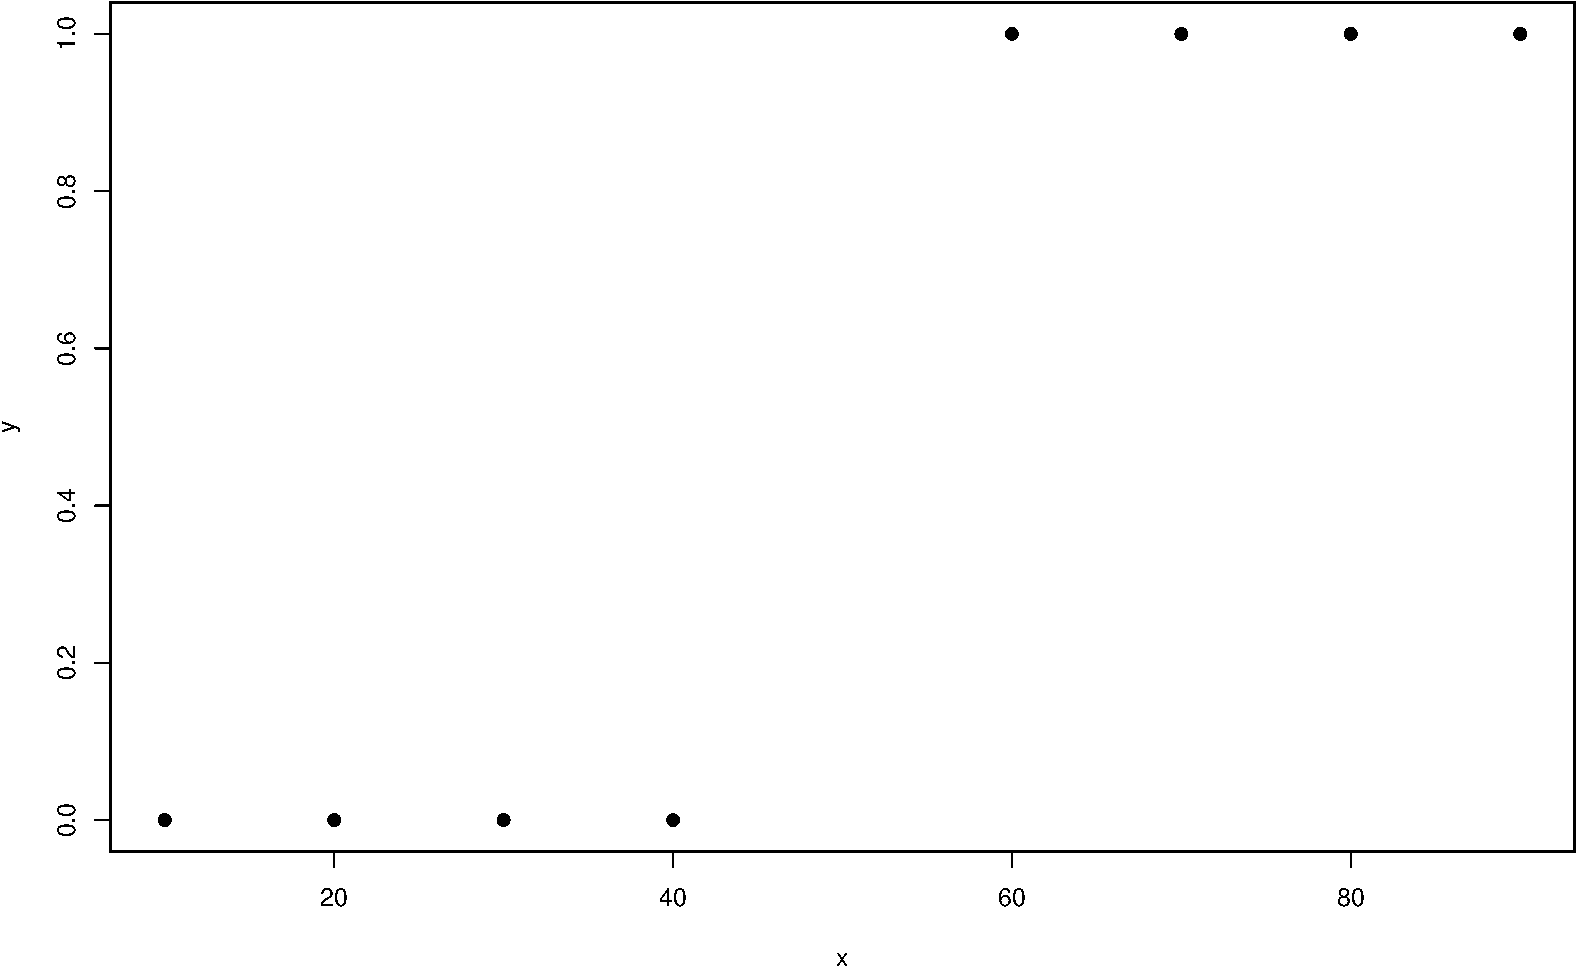
\includegraphics{week7_p2_files/figure-beamer/unnamed-chunk-1-1.pdf}
\end{frame}

\begin{frame}[fragile]{}
\protect\hypertarget{section-1}{}
Last time we demonstrated that there is a hyperplane which separates the
successes and failures.

\vspace{12pt}
\tiny

\begin{Shaded}
\begin{Highlighting}[]
\DocumentationTok{\#\# separation vector}
\NormalTok{b }\OtherTok{\textless{}{-}} \FunctionTok{c}\NormalTok{(}\SpecialCharTok{{-}}\DecValTok{50}\NormalTok{, }\DecValTok{1}\NormalTok{) }

\DocumentationTok{\#\# model matrix}
\NormalTok{M }\OtherTok{\textless{}{-}} \FunctionTok{cbind}\NormalTok{(}\DecValTok{1}\NormalTok{, x)}

\DocumentationTok{\#\# check condition}
\FunctionTok{cbind}\NormalTok{(M }\SpecialCharTok{\%*\%}\NormalTok{ b, y)}
\end{Highlighting}
\end{Shaded}

\begin{verbatim}
##          y
## [1,] -40 0
## [2,] -30 0
## [3,] -20 0
## [4,] -10 0
## [5,]  10 1
## [6,]  20 1
## [7,]  30 1
## [8,]  40 1
\end{verbatim}
\end{frame}

\begin{frame}[fragile]{}
\protect\hypertarget{section-2}{}
As we can see below the glm output is nonsense.

\vspace{12pt}
\tiny

\begin{Shaded}
\begin{Highlighting}[]
\NormalTok{m1 }\OtherTok{\textless{}{-}} \FunctionTok{glm}\NormalTok{(y }\SpecialCharTok{\textasciitilde{}}\NormalTok{ x, }\AttributeTok{family =} \StringTok{"binomial"}\NormalTok{)}
\end{Highlighting}
\end{Shaded}

\begin{verbatim}
## Warning: glm.fit: fitted probabilities numerically 0 or 1 occurred
\end{verbatim}

\begin{Shaded}
\begin{Highlighting}[]
\DocumentationTok{\#\# summary table}
\FunctionTok{summary}\NormalTok{(m1)}
\end{Highlighting}
\end{Shaded}

\begin{verbatim}
## 
## Call:
## glm(formula = y ~ x, family = "binomial")
## 
## Deviance Residuals: 
##        Min          1Q      Median          3Q         Max  
## -1.045e-05  -2.110e-08   0.000e+00   2.110e-08   1.045e-05  
## 
## Coefficients:
##               Estimate Std. Error z value Pr(>|z|)
## (Intercept)   -118.158 296046.174       0        1
## x                2.363   5805.939       0        1
## 
## (Dispersion parameter for binomial family taken to be 1)
## 
##     Null deviance: 1.1090e+01  on 7  degrees of freedom
## Residual deviance: 2.1827e-10  on 6  degrees of freedom
## AIC: 4
## 
## Number of Fisher Scoring iterations: 25
\end{verbatim}
\end{frame}

\begin{frame}{}
\protect\hypertarget{section-3}{}
The data exhibits complete degeneracy, and statistical inference is
essentially meaningless.

\vspace{12pt}

Luckily the computational checks have warned the user that a potential
problem has occurred.

\vspace{12pt}

Note that these warning messages do not describe what the problem is or
provide any guidance for how users should handle this problem.
\end{frame}

\begin{frame}[fragile]{}
\protect\hypertarget{section-4}{}
Morevover, these checks are purely computational and do not necessarily
imply that separation has occurred.

\vspace{12pt}
\tiny

\begin{Shaded}
\begin{Highlighting}[]
\NormalTok{w }\OtherTok{\textless{}{-}} \FunctionTok{c}\NormalTok{(x, }\FloatTok{1e3}\NormalTok{)}
\NormalTok{z }\OtherTok{\textless{}{-}} \FunctionTok{c}\NormalTok{(}\DecValTok{0}\NormalTok{,}\DecValTok{0}\NormalTok{,}\DecValTok{0}\NormalTok{,}\DecValTok{1}\NormalTok{,}\DecValTok{0}\NormalTok{,}\DecValTok{1}\NormalTok{,}\DecValTok{1}\NormalTok{,}\DecValTok{1}\NormalTok{,}\DecValTok{1}\NormalTok{)}
\NormalTok{m1\_alt }\OtherTok{\textless{}{-}} \FunctionTok{glm}\NormalTok{(z }\SpecialCharTok{\textasciitilde{}}\NormalTok{ w, }\AttributeTok{family =} \StringTok{"binomial"}\NormalTok{)}
\end{Highlighting}
\end{Shaded}

\begin{verbatim}
## Warning: glm.fit: fitted probabilities numerically 0 or 1 occurred
\end{verbatim}

\begin{Shaded}
\begin{Highlighting}[]
\FunctionTok{summary}\NormalTok{(m1\_alt)}
\end{Highlighting}
\end{Shaded}

\begin{verbatim}
## 
## Call:
## glm(formula = z ~ w, family = "binomial")
## 
## Deviance Residuals: 
##     Min       1Q   Median       3Q      Max  
## -1.5422  -0.4014   0.0000   0.4014   1.5422  
## 
## Coefficients:
##             Estimate Std. Error z value Pr(>|z|)
## (Intercept) -4.13039    2.74687  -1.504    0.133
## w            0.08261    0.05075   1.628    0.104
## 
## (Dispersion parameter for binomial family taken to be 1)
## 
##     Null deviance: 12.3653  on 8  degrees of freedom
## Residual deviance:  5.9245  on 7  degrees of freedom
## AIC: 9.9245
## 
## Number of Fisher Scoring iterations: 8
\end{verbatim}
\end{frame}

\begin{frame}[fragile]{}
\protect\hypertarget{section-5}{}
Notice that in the Agresti example the number of Fisher scoring
iterations is 25 (maximum allowable iterations). Look at what happens
when change the defaults:

\vspace{12pt}
\tiny

\begin{Shaded}
\begin{Highlighting}[]
\NormalTok{m2 }\OtherTok{\textless{}{-}} \FunctionTok{glm}\NormalTok{(y }\SpecialCharTok{\textasciitilde{}}\NormalTok{ x, }\AttributeTok{family =} \StringTok{"binomial"}\NormalTok{, }
          \AttributeTok{control =} \FunctionTok{list}\NormalTok{(}\AttributeTok{maxit =} \FloatTok{1e4}\NormalTok{, }\AttributeTok{epsilon =} \FloatTok{1e{-}100}\NormalTok{))}
\end{Highlighting}
\end{Shaded}

\begin{verbatim}
## Warning: glm.fit: fitted probabilities numerically 0 or 1 occurred
\end{verbatim}

\begin{Shaded}
\begin{Highlighting}[]
\FunctionTok{summary}\NormalTok{(m2)}
\end{Highlighting}
\end{Shaded}

\begin{verbatim}
## 
## Call:
## glm(formula = y ~ x, family = "binomial", control = list(maxit = 10000, 
##     epsilon = 1e-100))
## 
## Deviance Residuals: 
##        Min          1Q      Median          3Q         Max  
## -2.107e-08  -2.107e-08   0.000e+00   2.107e-08   2.107e-08  
## 
## Coefficients:
##               Estimate Std. Error z value Pr(>|z|)
## (Intercept) -1.546e+02  4.939e+07       0        1
## x            3.092e+00  8.664e+05       0        1
## 
## (Dispersion parameter for binomial family taken to be 1)
## 
##     Null deviance: 1.1090e+01  on 7  degrees of freedom
## Residual deviance: 3.5527e-15  on 6  degrees of freedom
## AIC: 4
## 
## Number of Fisher Scoring iterations: 33
\end{verbatim}
\end{frame}

\begin{frame}[fragile]{}
\protect\hypertarget{section-6}{}
Returning to the model fit with the default settings, we see large
canonical parameter estimates and mean value parameter estimates that
are at the boundary of the closure of their parameter space
\((0 < p < 1)\).

\vspace{12pt}

Informally, estimates are ``at infinity.'\,'

\vspace{12pt}
\tiny

\begin{Shaded}
\begin{Highlighting}[]
\DocumentationTok{\#\# submodel canonical parameter estimates}
\NormalTok{betahat }\OtherTok{\textless{}{-}}\NormalTok{ m1}\SpecialCharTok{$}\NormalTok{coefficients}
\NormalTok{betahat}
\end{Highlighting}
\end{Shaded}

\begin{verbatim}
## (Intercept)           x 
##  -118.15802     2.36316
\end{verbatim}

\begin{Shaded}
\begin{Highlighting}[]
\DocumentationTok{\#\# saturated model canonical parameter estimates}
\NormalTok{thetahat }\OtherTok{\textless{}{-}} \FunctionTok{as.numeric}\NormalTok{(M }\SpecialCharTok{\%*\%}\NormalTok{ betahat)}
\NormalTok{thetahat}
\end{Highlighting}
\end{Shaded}

\begin{verbatim}
## [1] -94.52642 -70.89481 -47.26321 -23.63160  23.63160  47.26321  70.89481
## [8]  94.52642
\end{verbatim}

\begin{Shaded}
\begin{Highlighting}[]
\DocumentationTok{\#\# saturated model mean value parameter estimates}
\NormalTok{phat }\OtherTok{\textless{}{-}} \FunctionTok{predict}\NormalTok{(m1, }\AttributeTok{type =} \StringTok{"response"}\NormalTok{)}
\NormalTok{phat}
\end{Highlighting}
\end{Shaded}

\begin{verbatim}
##            1            2            3            4            5            6 
## 2.220446e-16 2.220446e-16 2.220446e-16 5.456633e-11 1.000000e+00 1.000000e+00 
##            7            8 
## 1.000000e+00 1.000000e+00
\end{verbatim}
\end{frame}

\begin{frame}{Canonical statistic on the boundary of its support}
\protect\hypertarget{canonical-statistic-on-the-boundary-of-its-support}{}
Recall that the submodel can be written as \[
  \langle y, M\beta \rangle - c(M\beta) = \langle M^Ty, \beta \rangle - c_\beta(\beta)
\] \vspace{12pt} Also notice that the observed value of the canonical
statistic \(M^Ty\) for the above submodel is on the boundary of the
support of values for \(M^TY\).

\vspace{12pt}

This implies that the MLE does not exist in the traditional sense. See
\href{https://projecteuclid.org/euclid.ejs/1239716414}{Geyer (2009)} for
technical details that are beyond the scope of this course).
\end{frame}

\begin{frame}{}
\protect\hypertarget{section-7}{}
\begin{center}
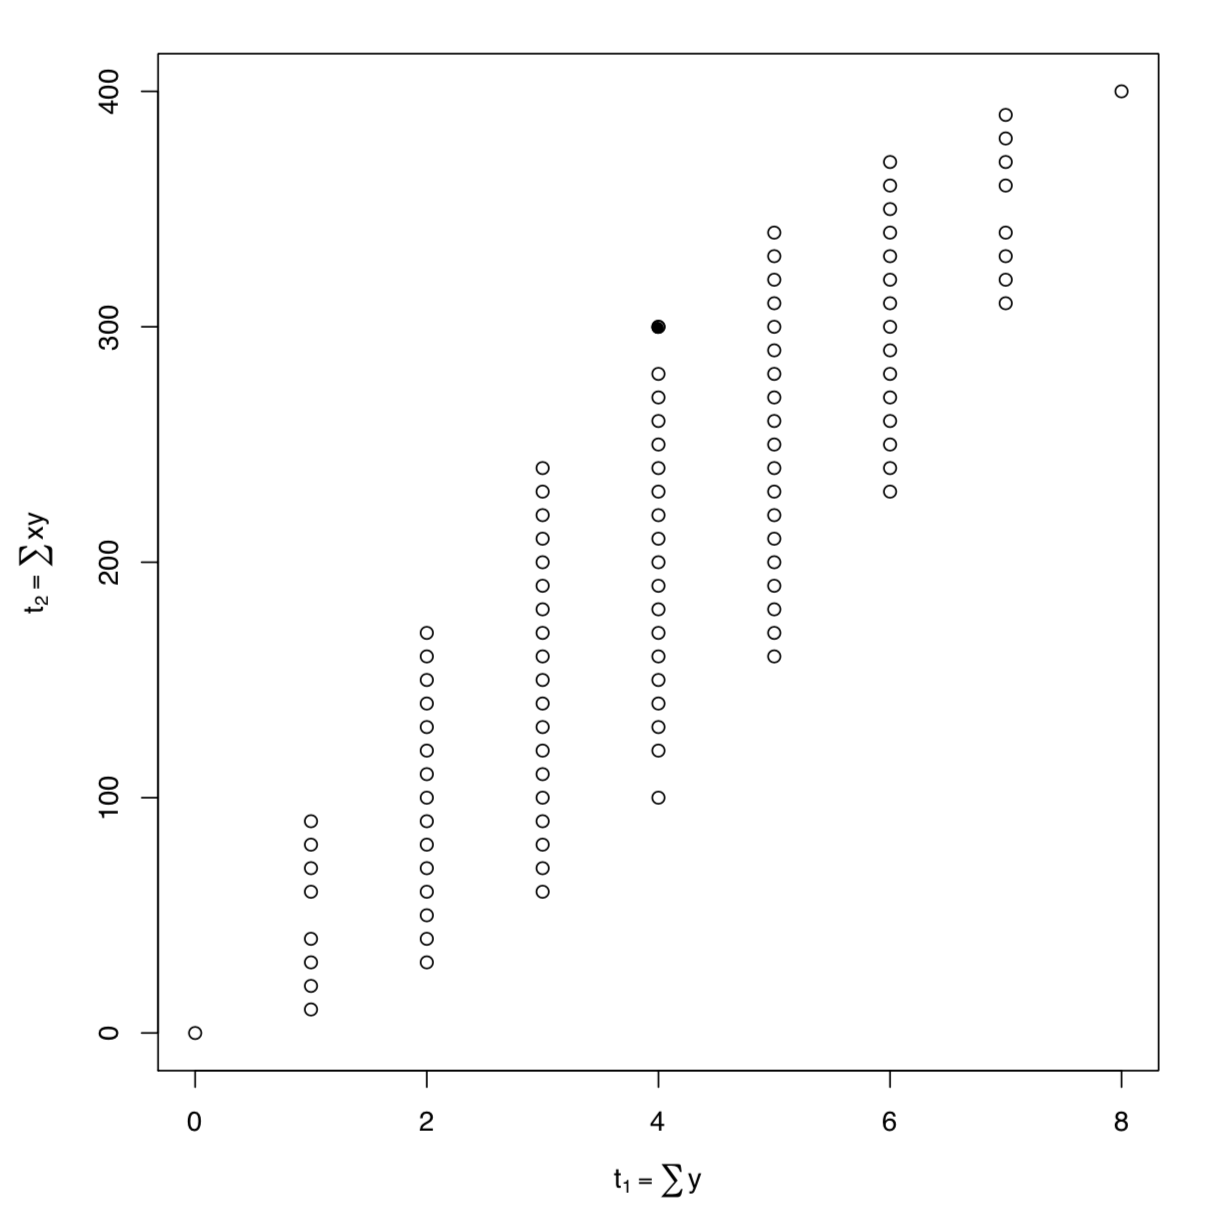
\includegraphics[width = 0.75\textwidth]{boundaryMtY.png}
\end{center}
\end{frame}

\begin{frame}[fragile]{}
\protect\hypertarget{section-8}{}
Note that, by the observed equals expected property, \(M^Ty\) is the MLE
of the submodel mean-value parameter vector. The variance of the
submodel canonical statistic is the Fisher information matrix.

\vspace{12pt}

We now use R scripts to compute the Fisher information matrix. An
eigenvector decomposition reveals that the Fisher information matrix is
numerically singular.

\vspace{12pt}
\tiny

\begin{Shaded}
\begin{Highlighting}[]
\NormalTok{invFI }\OtherTok{\textless{}{-}} \FunctionTok{vcov}\NormalTok{(m1)}
\NormalTok{FI }\OtherTok{\textless{}{-}} \FunctionTok{solve}\NormalTok{(invFI)}
\FunctionTok{eigen}\NormalTok{(FI)}
\end{Highlighting}
\end{Shaded}

\begin{verbatim}
## eigen() decomposition
## $values
## [1] 7.715655e-07 1.140566e-11
## 
## $vectors
##            [,1]        [,2]
## [1,] 0.01922747 -0.99981514
## [2,] 0.99981514  0.01922747
\end{verbatim}
\end{frame}

\begin{frame}{}
\protect\hypertarget{section-9}{}
This implies that \(\widehat{\text{Var}}(M^TY) = 0\).

\vspace{12pt}

Therefore, the MLE solution to this problem is that the observed data
which are on the boundary are the only possible data that could have
occurred.

\vspace{12pt}

Of course, these are estimates and not actual parameters. The problem is
how to make inferential statements about model parameters given this
degeneracy.
\end{frame}

\begin{frame}[fragile]{Inference in the complete separation setting}
\protect\hypertarget{inference-in-the-complete-separation-setting}{}
The exponential family in this example is completely degenerate. The MLE
does not exist in the traditional sense, but may (does) exist in the
completion of the exponential family (the set which includes all
exponential family distributions and all limits of distributions).

\vspace{12pt}

Conventional maximum likelihood computations come close, in a sense, to
finding the MLE in the completion of the exponential family. They go
uphill on the likelihood function until they meet their convergence
criteria and stop.

\vspace{12pt}
\tiny

\begin{Shaded}
\begin{Highlighting}[]
\NormalTok{asymptote }\OtherTok{\textless{}{-}} \FunctionTok{t}\NormalTok{(}\FunctionTok{sapply}\NormalTok{(}\DecValTok{1}\SpecialCharTok{:}\DecValTok{30}\NormalTok{, }\ControlFlowTok{function}\NormalTok{(iter)\{}
\NormalTok{  m1 }\OtherTok{\textless{}{-}} \FunctionTok{glm}\NormalTok{(y }\SpecialCharTok{\textasciitilde{}}\NormalTok{ x, }\AttributeTok{family =} \StringTok{"binomial"}\NormalTok{, }\AttributeTok{control =} \FunctionTok{list}\NormalTok{(}\AttributeTok{maxit =}\NormalTok{ iter, }\AttributeTok{epsilon =} \FloatTok{1e{-}20}\NormalTok{))}
  \FunctionTok{c}\NormalTok{(}\FunctionTok{sqrt}\NormalTok{(}\FunctionTok{log}\NormalTok{(}\FunctionTok{crossprod}\NormalTok{(}\FunctionTok{coef}\NormalTok{(m1)))), }\FunctionTok{logLik}\NormalTok{(m1))}
\NormalTok{\}))}
\NormalTok{asymptote }\OtherTok{\textless{}{-}} \FunctionTok{as.data.frame}\NormalTok{(asymptote)}
\end{Highlighting}
\end{Shaded}
\end{frame}

\begin{frame}{}
\protect\hypertarget{section-10}{}
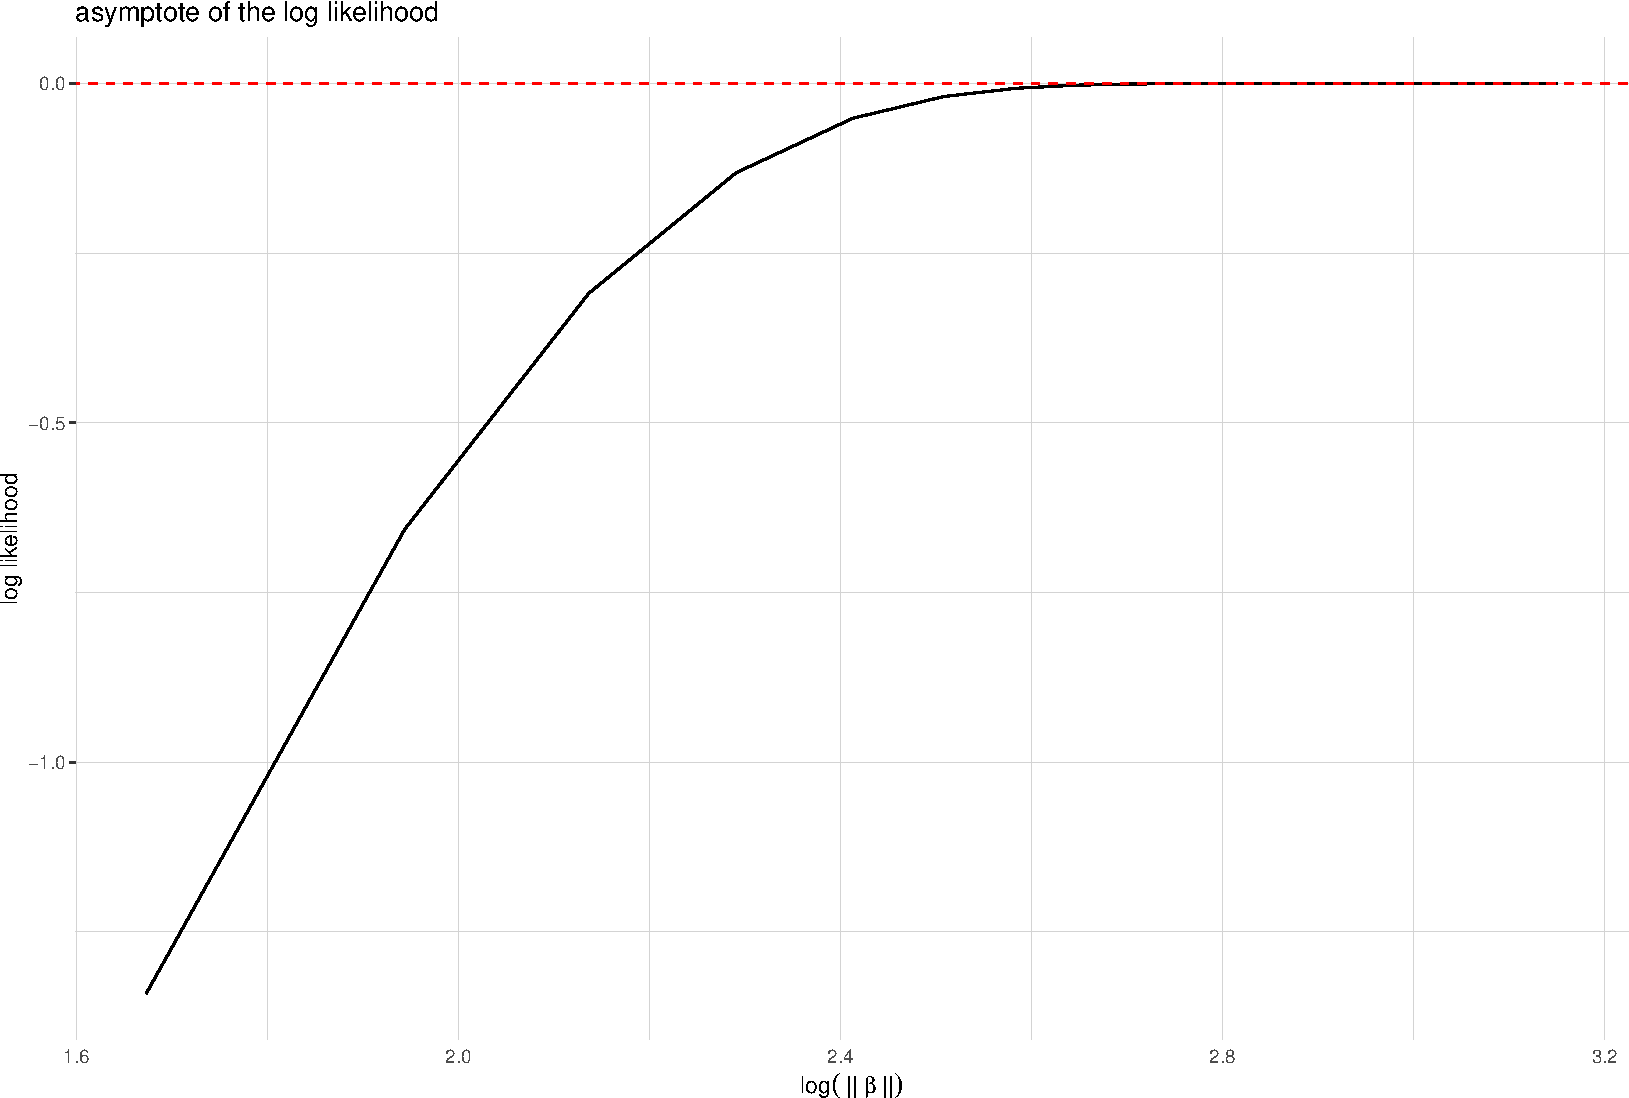
\includegraphics{week7_p2_files/figure-beamer/unnamed-chunk-9-1.pdf}
\end{frame}

\begin{frame}{}
\protect\hypertarget{section-11}{}
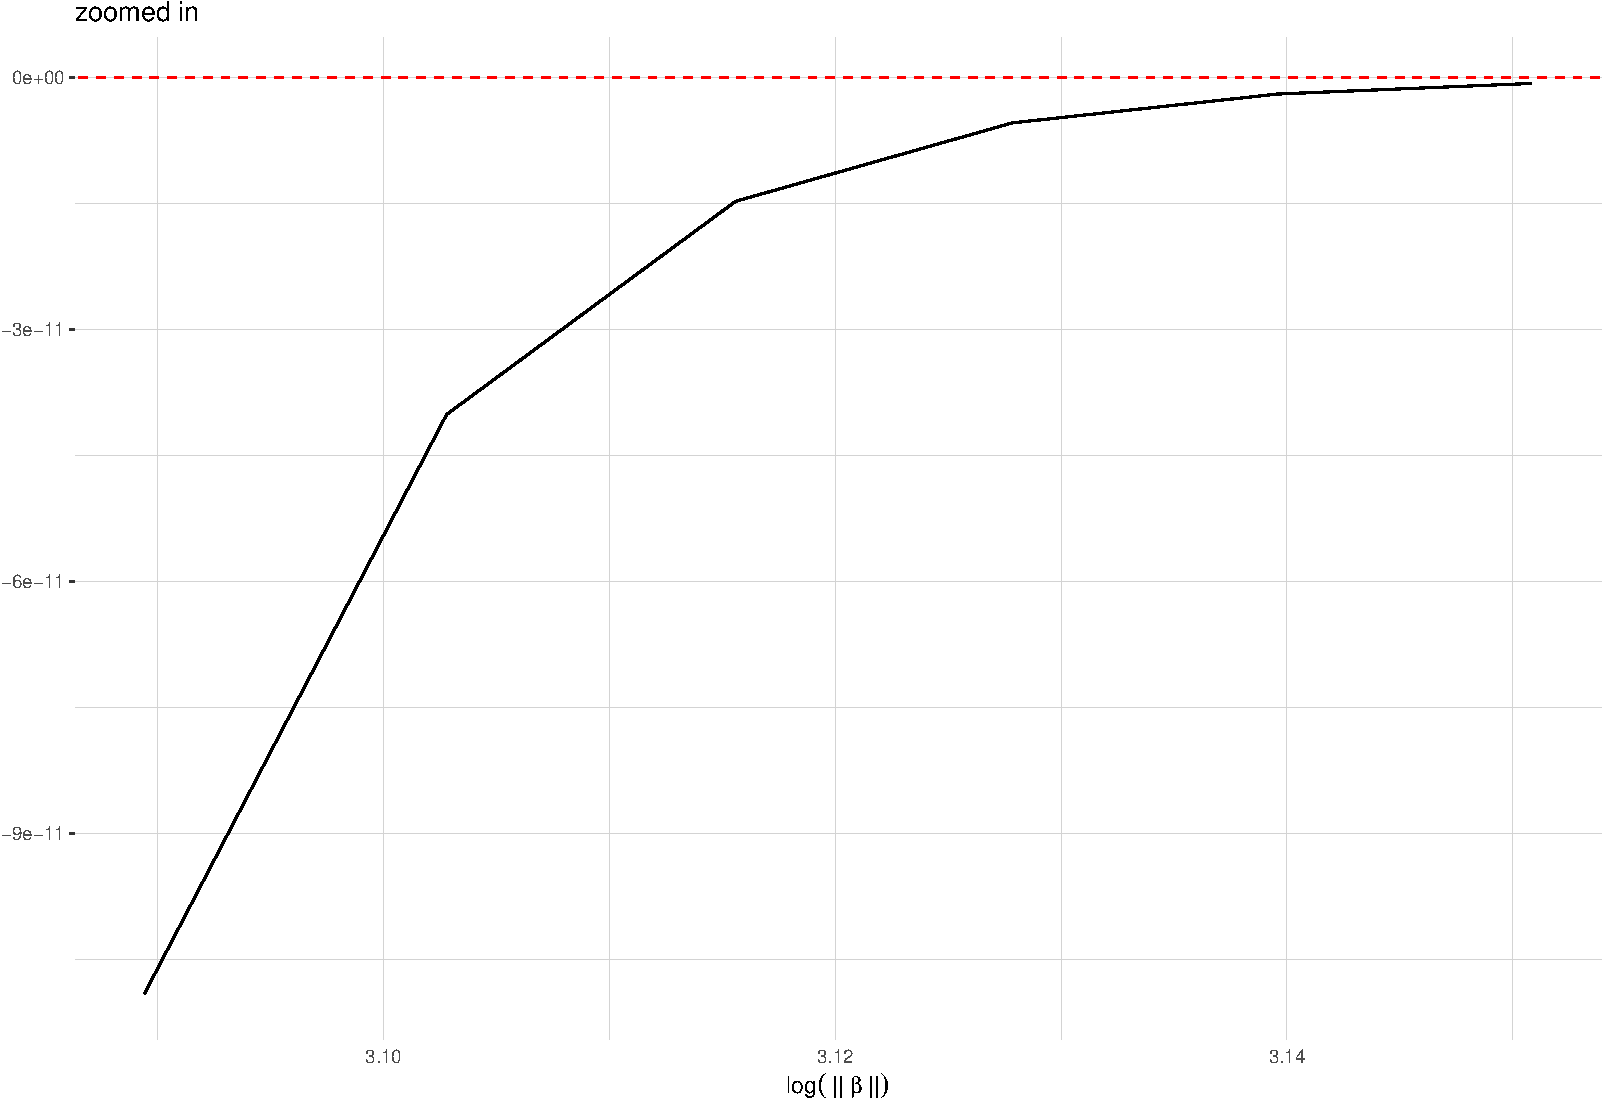
\includegraphics{week7_p2_files/figure-beamer/unnamed-chunk-10-1.pdf}
\end{frame}

\begin{frame}{}
\protect\hypertarget{section-12}{}
At this point, canonical parameter estimates \(\hat\theta\) and
\(\hat\beta\) are still infinitely far away from the MLE in the
completion.

\vspace{12pt}

But mean value parameter estimates \(\hat\mu\) are close to the MLE in
the completion, and the log likelihood is nearly maximized.

\vspace{12pt}

And the corresponding probability distributions are close in total
variation norm to the MLE probability distribution in the completion.
\end{frame}

\begin{frame}[fragile]{Software and return to Agresti example}
\protect\hypertarget{software-and-return-to-agresti-example}{}
The \texttt{inference} function in the R package \texttt{glmdr}
determines one-sided confidence intervals for mean value parameters
corresponding to response values that are constrained to their observed
values \(y_I\)

\vspace{12pt}
\tiny

\begin{Shaded}
\begin{Highlighting}[]
\FunctionTok{library}\NormalTok{(glmdr)}
\end{Highlighting}
\end{Shaded}

\vspace{12pt}
\normalsize

\begin{itemize}
\tightlist
\item
  See the \texttt{glmdr} directory in the stat528resources repo. You
  will have to install the package locally
\item
  The \texttt{glmdr} package currently only works for logistic,
  binomial, and Poisson regression.
\end{itemize}
\end{frame}

\begin{frame}[fragile]{}
\protect\hypertarget{section-13}{}
We now fit the logistic regression model using the \texttt{glmdr}
fitting function instead of \texttt{glm}. The user is prompted with a
description of the problem which provides guidance on how to handle the
problem.

\vspace{12pt}
\tiny

\begin{Shaded}
\begin{Highlighting}[]
\NormalTok{m\_glmdr }\OtherTok{\textless{}{-}} \FunctionTok{glmdr}\NormalTok{(y }\SpecialCharTok{\textasciitilde{}}\NormalTok{ x)}

\DocumentationTok{\#\# summary information}
\FunctionTok{summary}\NormalTok{(m\_glmdr)}
\end{Highlighting}
\end{Shaded}

\begin{verbatim}
## MLE exists in Barndorff-Nielsen completion
## it is completely degenerate
## the MLE says the response actually observed is the only
## possible value that could ever be observed
\end{verbatim}

\begin{verbatim}
## $overview
## NULL
## 
## $type
## [1] "degenerate"
## 
## $linearity
## [1] FALSE FALSE FALSE FALSE FALSE FALSE FALSE FALSE
## 
## attr(,"class")
## [1] "summary.glmdr"
\end{verbatim}
\end{frame}

\begin{frame}[fragile]{}
\protect\hypertarget{section-14}{}
We then use the \texttt{inference} function to obtain one sided
confidence intervals for mean-value parameters corresponding to
components \(Y_I\) that are constrained to be their observed values.

\vspace{12pt}
\tiny

\begin{Shaded}
\begin{Highlighting}[]
\DocumentationTok{\#\# one{-}sided CIs}
\NormalTok{CIs }\OtherTok{\textless{}{-}} \FunctionTok{inference}\NormalTok{(m\_glmdr)}
\NormalTok{CIs}
\end{Highlighting}
\end{Shaded}

\begin{verbatim}
##       lower     upper
## 1 0.0000000 0.2852500
## 2 0.0000000 0.3940359
## 3 0.0000000 0.5708292
## 4 0.0000000 0.9500000
## 5 0.0500000 1.0000000
## 6 0.4291708 1.0000000
## 7 0.6059641 1.0000000
## 8 0.7147500 1.0000000
\end{verbatim}
\end{frame}

\begin{frame}{}
\protect\hypertarget{section-15}{}
\begin{center}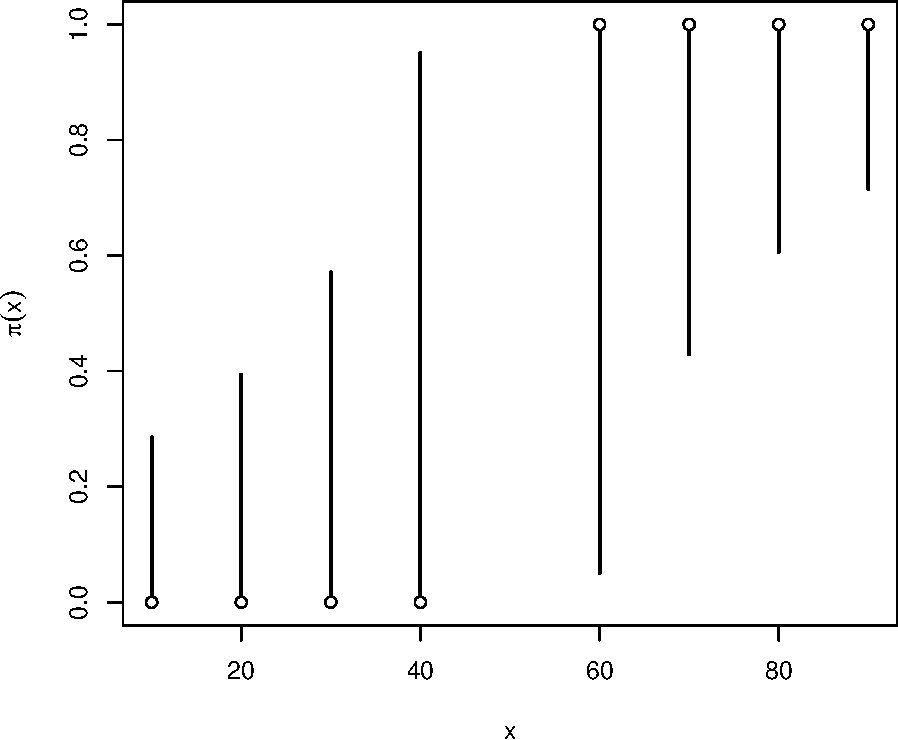
\includegraphics{week7_p2_files/figure-beamer/unnamed-chunk-14-1} \end{center}
\end{frame}

\begin{frame}{Commentary on Agresti}
\protect\hypertarget{commentary-on-agresti}{}
The \(n = 8\) data point example that we analyzed comes from Section
6.5.1 in Agresti.

\vspace{12pt}

However, this textbook provides no model based inferential solution to
this problem.

\vspace{12pt}

This week, we provided such a solution that exists within the
exponential family modeling and maximum likelihood estimation paradigms.

\vspace{12pt}

To be fair to Agresti, ``solutions'' to complete separation are
discussed in Sections 7.4.8.
\end{frame}

\begin{frame}{Not completely degenerate}
\protect\hypertarget{not-completely-degenerate}{}
In the Agresti example we noticed that the estimated Fisher information
matrix was completely degenerate. T

\vspace{12pt}

his need not be so in generality, the Fisher information matrix can
exhibit partial degeneracy.

\vspace{12pt}

When this is so the limiting conditional model (LCM) is not completely
degenerate, data pairs \((y_i,x_i)\) corresponding to response vectors
which are left unconstrained form the LCM and parameter estimation can
be conducted in a traditional manner.

\vspace{12pt}

We will now explore an example where with partial degeneracy.
\end{frame}

\begin{frame}[fragile]{Endometrial example}
\protect\hypertarget{endometrial-example}{}
We will consider the endometrial example in which the a histology grade
and risk factors for 79 cases of endometrial cancer are analyzed. the
variables are:

\begin{itemize}
\tightlist
\item
  \textbf{NV}: neovasculization with coding 0 for absent and 1 for
  present
\item
  \textbf{PI}: pulsality index of arteria uterina
\item
  \textbf{EH}: endometrium heigh
\item
  \textbf{HG}: histology grade with coding 0 for low grade and 1 for
  high grade
\end{itemize}

\vspace{12pt}
\tiny

\begin{Shaded}
\begin{Highlighting}[]
\FunctionTok{library}\NormalTok{(enrichwith)}
\FunctionTok{data}\NormalTok{(endometrial)}
\FunctionTok{head}\NormalTok{(endometrial, }\DecValTok{3}\NormalTok{)}
\end{Highlighting}
\end{Shaded}

\begin{verbatim}
##   NV PI   EH HG
## 1  0 13 1.64  0
## 2  0 16 2.26  0
## 3  0  8 3.14  0
\end{verbatim}
\end{frame}

\begin{frame}[fragile]{}
\protect\hypertarget{section-16}{}
We begin with a standard logistic regression fit.

\vspace{12pt}
\tiny

\begin{Shaded}
\begin{Highlighting}[]
\NormalTok{m }\OtherTok{\textless{}{-}} \FunctionTok{glm}\NormalTok{(HG }\SpecialCharTok{\textasciitilde{}}\NormalTok{ ., }\AttributeTok{data =}\NormalTok{ endometrial, }\AttributeTok{family =} \StringTok{"binomial"}\NormalTok{, }
         \AttributeTok{x =} \ConstantTok{TRUE}\NormalTok{, }\AttributeTok{y =} \ConstantTok{TRUE}\NormalTok{)}
\FunctionTok{summary}\NormalTok{(m)}
\end{Highlighting}
\end{Shaded}

\begin{verbatim}
## 
## Call:
## glm(formula = HG ~ ., family = "binomial", data = endometrial, 
##     x = TRUE, y = TRUE)
## 
## Deviance Residuals: 
##      Min        1Q    Median        3Q       Max  
## -1.50137  -0.64108  -0.29432   0.00016   2.72777  
## 
## Coefficients:
##               Estimate Std. Error z value Pr(>|z|)    
## (Intercept)    4.30452    1.63730   2.629 0.008563 ** 
## NV            18.18556 1715.75089   0.011 0.991543    
## PI            -0.04218    0.04433  -0.952 0.341333    
## EH            -2.90261    0.84555  -3.433 0.000597 ***
## ---
## Signif. codes:  0 '***' 0.001 '**' 0.01 '*' 0.05 '.' 0.1 ' ' 1
## 
## (Dispersion parameter for binomial family taken to be 1)
## 
##     Null deviance: 104.903  on 78  degrees of freedom
## Residual deviance:  55.393  on 75  degrees of freedom
## AIC: 63.393
## 
## Number of Fisher Scoring iterations: 17
\end{verbatim}
\end{frame}

\begin{frame}[fragile]{}
\protect\hypertarget{section-17}{}
We observe \textbf{quasi-complete separation} in NV (a categorical
variable with two levels), where we note that a 2 × 2 contingency table
with an empty (zero) cell is an example of quasi-complete separation.

\vspace{12pt}
\tiny

\begin{Shaded}
\begin{Highlighting}[]
\NormalTok{b }\OtherTok{\textless{}{-}} \FunctionTok{c}\NormalTok{(}\DecValTok{0}\NormalTok{,}\DecValTok{1}\NormalTok{,}\DecValTok{0}\NormalTok{,}\DecValTok{0}\NormalTok{)}
\FunctionTok{library}\NormalTok{(data.table)}
\end{Highlighting}
\end{Shaded}

\begin{verbatim}
## 
## Attaching package: 'data.table'
\end{verbatim}

\begin{verbatim}
## The following objects are masked from 'package:dplyr':
## 
##     between, first, last
\end{verbatim}

\begin{verbatim}
## The following object is masked from 'package:purrr':
## 
##     transpose
\end{verbatim}

\begin{Shaded}
\begin{Highlighting}[]
\NormalTok{foo }\OtherTok{\textless{}{-}} \FunctionTok{setDT}\NormalTok{(}\FunctionTok{as.data.frame}\NormalTok{(}\FunctionTok{cbind}\NormalTok{(m}\SpecialCharTok{$}\NormalTok{y, m}\SpecialCharTok{$}\NormalTok{x }\SpecialCharTok{\%*\%}\NormalTok{ b)))}
\FunctionTok{colnames}\NormalTok{(foo) }\OtherTok{\textless{}{-}} \FunctionTok{c}\NormalTok{(}\StringTok{"y"}\NormalTok{, }\StringTok{"sep"}\NormalTok{)}
\NormalTok{foo[, .(.N), by }\OtherTok{=} \FunctionTok{c}\NormalTok{(}\StringTok{"y"}\NormalTok{, }\StringTok{"sep"}\NormalTok{)]}
\end{Highlighting}
\end{Shaded}

\begin{verbatim}
##    y sep  N
## 1: 0   0 49
## 2: 1   0 17
## 3: 1   1 13
\end{verbatim}
\end{frame}

\begin{frame}[fragile]{}
\protect\hypertarget{section-18}{}
We now use \texttt{glmdr} to do our fitting. The user is prompted with a
description of the problem which provides guidance on how to handle the
problem.

\vspace{12pt}
\tiny

\begin{Shaded}
\begin{Highlighting}[]
\NormalTok{m\_glmdr }\OtherTok{\textless{}{-}} \FunctionTok{glmdr}\NormalTok{(HG }\SpecialCharTok{\textasciitilde{}}\NormalTok{ ., }\AttributeTok{data =}\NormalTok{ endometrial, }\AttributeTok{family =} \StringTok{"binomial"}\NormalTok{)}
\FunctionTok{summary}\NormalTok{(m\_glmdr)}
\end{Highlighting}
\end{Shaded}

\begin{verbatim}
## MLE exists in Barndorff-Nielsen completion
## it is conditional on components of the response
## corresponding to object$linearity == FALSE being
## conditioned on their observed values
\end{verbatim}

\begin{verbatim}
## $overview
## NULL
## 
## $type
## [1] "lcm"
## 
## $summary
## 
## Call:
## stats::glm(formula = HG ~ ., family = "binomial", data = endometrial, 
##     subset = c("1", "2", "3", "4", "5", "6", "7", "8", "9", "10", 
##     "11", "12", "13", "14", "15", "16", "17", "18", "19", "20", 
##     "21", "27", "28", "29", "30", "31", "32", "33", "34", "35", 
##     "36", "37", "38", "39", "40", "41", "42", "43", "44", "45", 
##     "46", "47", "52", "53", "54", "55", "56", "57", "58", "59", 
##     "60", "61", "62", "63", "64", "65", "66", "67", "68", "69", 
##     "70", "72", "73", "74", "77", "79"), x = TRUE, y = TRUE)
## 
## Deviance Residuals: 
##     Min       1Q   Median       3Q      Max  
## -1.5014  -0.6634  -0.3856   0.2126   2.7278  
## 
## Coefficients: (1 not defined because of singularities)
##             Estimate Std. Error z value Pr(>|z|)    
## (Intercept)  4.30452    1.63720   2.629 0.008559 ** 
## NV                NA         NA      NA       NA    
## PI          -0.04218    0.04433  -0.952 0.341310    
## EH          -2.90261    0.84549  -3.433 0.000597 ***
## ---
## Signif. codes:  0 '***' 0.001 '**' 0.01 '*' 0.05 '.' 0.1 ' ' 1
## 
## (Dispersion parameter for binomial family taken to be 1)
## 
##     Null deviance: 75.307  on 65  degrees of freedom
## Residual deviance: 55.393  on 63  degrees of freedom
## AIC: 61.393
## 
## Number of Fisher Scoring iterations: 5
## 
## 
## $linearity
##     1     2     3     4     5     6     7     8     9    10    11    12    13 
##  TRUE  TRUE  TRUE  TRUE  TRUE  TRUE  TRUE  TRUE  TRUE  TRUE  TRUE  TRUE  TRUE 
##    14    15    16    17    18    19    20    21    22    23    24    25    26 
##  TRUE  TRUE  TRUE  TRUE  TRUE  TRUE  TRUE  TRUE FALSE FALSE FALSE FALSE FALSE 
##    27    28    29    30    31    32    33    34    35    36    37    38    39 
##  TRUE  TRUE  TRUE  TRUE  TRUE  TRUE  TRUE  TRUE  TRUE  TRUE  TRUE  TRUE  TRUE 
##    40    41    42    43    44    45    46    47    48    49    50    51    52 
##  TRUE  TRUE  TRUE  TRUE  TRUE  TRUE  TRUE  TRUE FALSE FALSE FALSE FALSE  TRUE 
##    53    54    55    56    57    58    59    60    61    62    63    64    65 
##  TRUE  TRUE  TRUE  TRUE  TRUE  TRUE  TRUE  TRUE  TRUE  TRUE  TRUE  TRUE  TRUE 
##    66    67    68    69    70    71    72    73    74    75    76    77    78 
##  TRUE  TRUE  TRUE  TRUE  TRUE FALSE  TRUE  TRUE  TRUE FALSE FALSE  TRUE FALSE 
##    79 
##  TRUE 
## 
## attr(,"class")
## [1] "summary.glmdr"
\end{verbatim}
\end{frame}

\begin{frame}[fragile]{}
\protect\hypertarget{section-19}{}
The summary table is strange. The variable driving quasi-complete
separation has been dropped from consideration.

\vspace{12pt}

We only observe partially degeneracy of Fisher Information (the variance
matrix for the submodel canonical statistic).

\vspace{12pt}
\tiny

\begin{Shaded}
\begin{Highlighting}[]
\FunctionTok{solve}\NormalTok{(}\FunctionTok{vcov}\NormalTok{(m))}
\end{Highlighting}
\end{Shaded}

\begin{verbatim}
##              (Intercept)           NV           PI           EH
## (Intercept) 8.971281e+00 3.396969e-07 1.499626e+02 1.334686e+01
## NV          3.396969e-07 3.396969e-07 8.916423e-06 3.821298e-07
## PI          1.499626e+02 8.916423e-06 3.045253e+03 2.164762e+02
## EH          1.334686e+01 3.821298e-07 2.164762e+02 2.133680e+01
\end{verbatim}
\end{frame}

\begin{frame}[fragile]{}
\protect\hypertarget{section-20}{}
The reason for this strangeness is beyond the scope of this course. The
interested reader can check out Lemma 1 and Corollary 1 in Section
6.1.3. in
\href{https://projecteuclid.org/journals/electronic-journal-of-statistics/volume-15/issue-1/Computationally-efficient-likelihood-inference-in-exponential-families-when-the-maximum/10.1214/21-EJS1815.full}{Eck
and Geyer (2021)}.

\vspace{12pt}

We now investigate what is going on under the hood.

\vspace{12pt}
\tiny

\begin{Shaded}
\begin{Highlighting}[]
\NormalTok{asymptote }\OtherTok{\textless{}{-}} \FunctionTok{t}\NormalTok{(}\FunctionTok{sapply}\NormalTok{(}\DecValTok{1}\SpecialCharTok{:}\DecValTok{30}\NormalTok{, }\ControlFlowTok{function}\NormalTok{(iter)\{}
\NormalTok{  m\_test }\OtherTok{\textless{}{-}} \FunctionTok{glm}\NormalTok{(HG }\SpecialCharTok{\textasciitilde{}}\NormalTok{ ., }\AttributeTok{family =} \StringTok{"binomial"}\NormalTok{, }\AttributeTok{data =}\NormalTok{ endometrial, }
                \AttributeTok{control =} \FunctionTok{list}\NormalTok{(}\AttributeTok{maxit =}\NormalTok{ iter, }\AttributeTok{epsilon =} \FloatTok{1e{-}20}\NormalTok{))}
  \FunctionTok{c}\NormalTok{(}\FunctionTok{sqrt}\NormalTok{(}\FunctionTok{log}\NormalTok{(}\FunctionTok{crossprod}\NormalTok{(}\FunctionTok{coef}\NormalTok{(m\_test)))), }\FunctionTok{logLik}\NormalTok{(m\_test), }\FunctionTok{coef}\NormalTok{(m\_test))}
\NormalTok{\}))}
\NormalTok{asymptote }\OtherTok{\textless{}{-}} \FunctionTok{as.data.frame}\NormalTok{(asymptote)}
\end{Highlighting}
\end{Shaded}
\end{frame}

\begin{frame}{}
\protect\hypertarget{section-21}{}
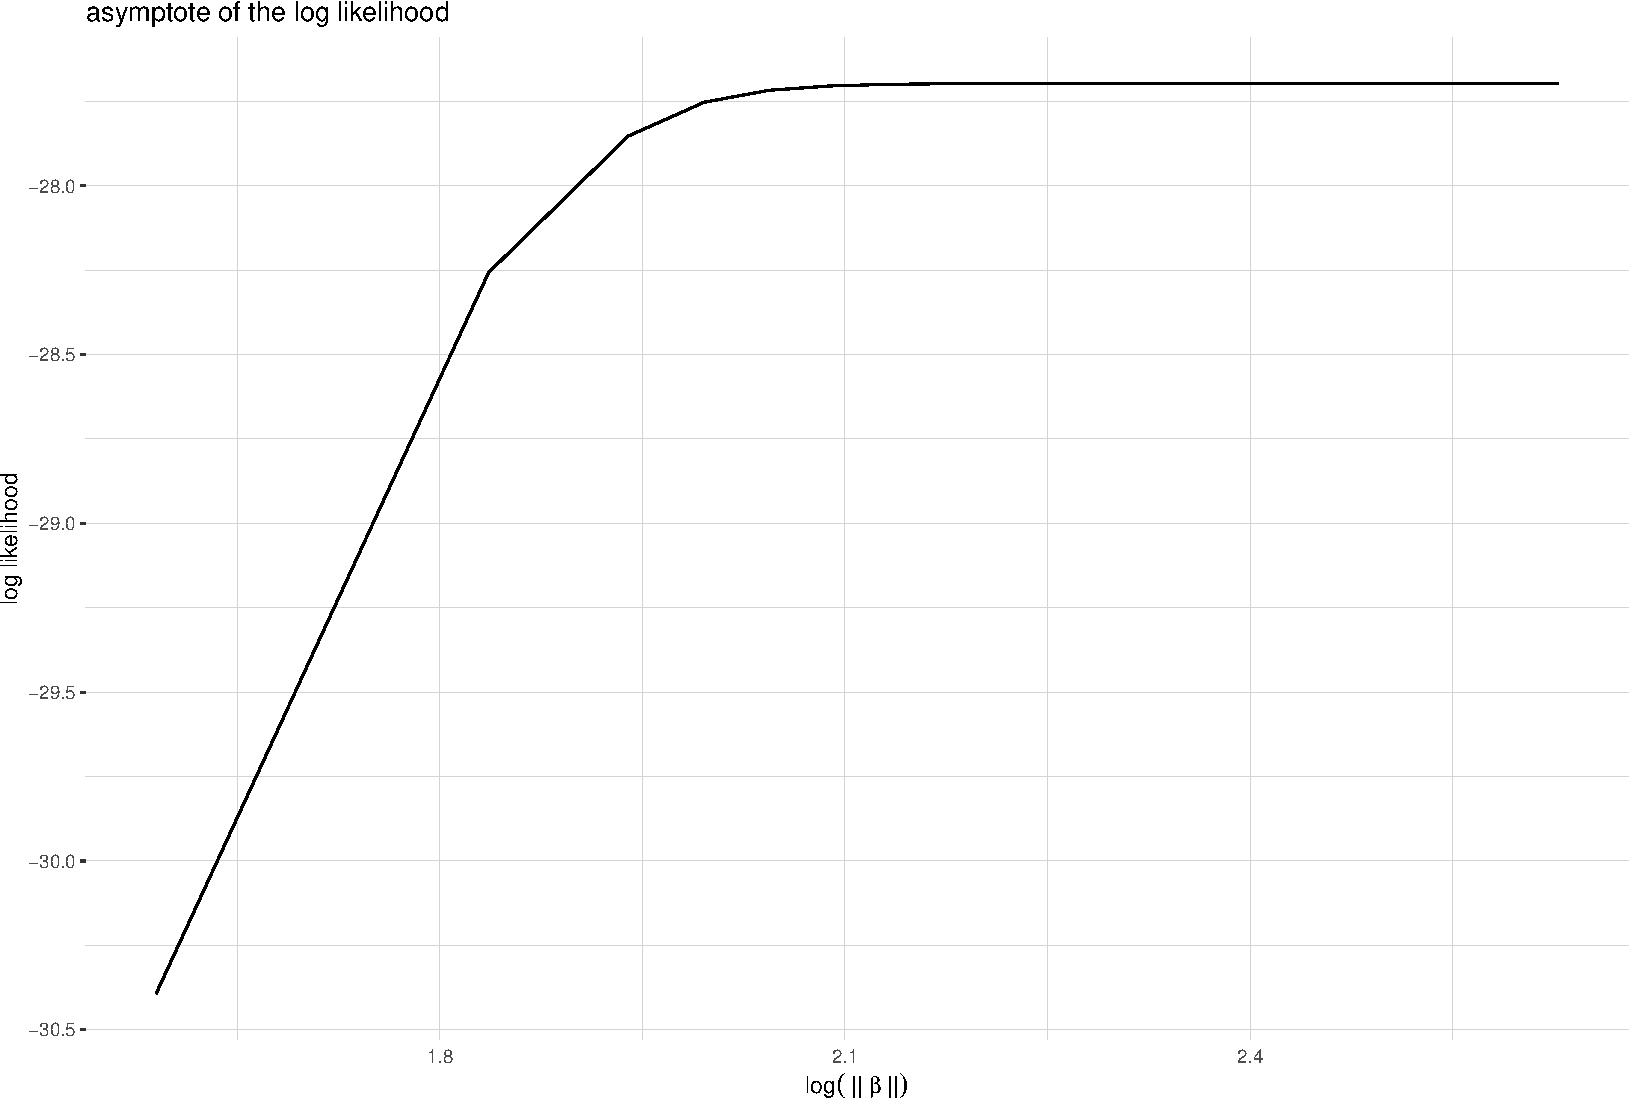
\includegraphics{week7_p2_files/figure-beamer/unnamed-chunk-21-1.pdf}
\end{frame}

\begin{frame}{}
\protect\hypertarget{section-22}{}
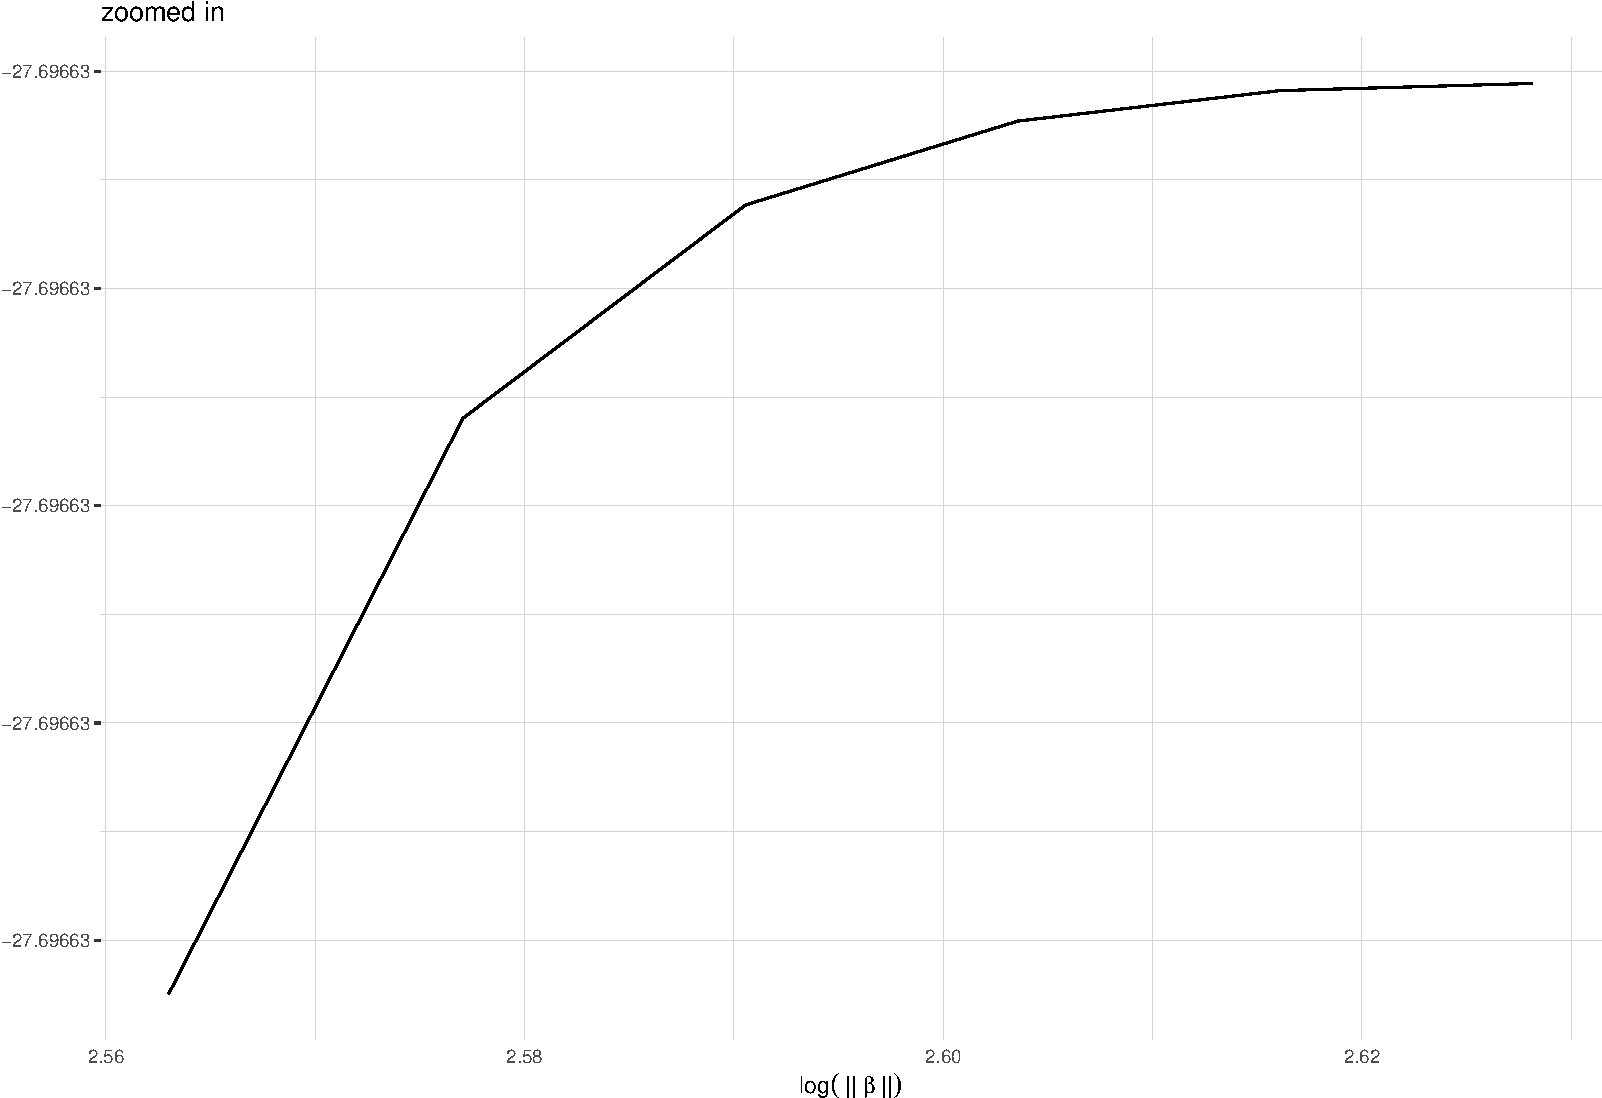
\includegraphics{week7_p2_files/figure-beamer/unnamed-chunk-22-1.pdf}
\end{frame}

\begin{frame}[fragile]{}
\protect\hypertarget{section-23}{}
\tiny

\begin{Shaded}
\begin{Highlighting}[]
\NormalTok{asymptote }\SpecialCharTok{\%\textgreater{}\%} \FunctionTok{mutate}\NormalTok{(}\AttributeTok{iter =} \DecValTok{1}\SpecialCharTok{:}\DecValTok{30}\NormalTok{) }\SpecialCharTok{\%\textgreater{}\%} 
\NormalTok{  dplyr}\SpecialCharTok{::}\FunctionTok{select}\NormalTok{(}\DecValTok{3}\SpecialCharTok{:}\DecValTok{6}\NormalTok{) }\SpecialCharTok{\%\textgreater{}\%} \FunctionTok{as.data.frame}\NormalTok{()}
\end{Highlighting}
\end{Shaded}

\begin{verbatim}
##    (Intercept)        NV          PI        EH
## 1     2.090959  2.355064 -0.02213019 -1.612126
## 2     3.599433  3.144596 -0.03327115 -2.502950
## 3     4.203858  4.148140 -0.04030884 -2.852134
## 4     4.300150  5.172614 -0.04205976 -2.900986
## 5     4.304349  6.181031 -0.04217827 -2.902550
## 6     4.304501  7.183901 -0.04218293 -2.902599
## 7     4.304516  8.184948 -0.04218334 -2.902605
## 8     4.304517  9.185332 -0.04218340 -2.902606
## 9     4.304518 10.185474 -0.04218340 -2.902606
## 10    4.304518 11.185526 -0.04218340 -2.902606
## 11    4.304518 12.185545 -0.04218340 -2.902606
## 12    4.304518 13.185552 -0.04218340 -2.902606
## 13    4.304518 14.185554 -0.04218340 -2.902606
## 14    4.304518 15.185555 -0.04218340 -2.902606
## 15    4.304518 16.185556 -0.04218340 -2.902606
## 16    4.304518 17.185556 -0.04218340 -2.902606
## 17    4.304518 18.185556 -0.04218340 -2.902606
## 18    4.304518 19.185556 -0.04218340 -2.902606
## 19    4.304518 20.185556 -0.04218340 -2.902606
## 20    4.304518 21.185556 -0.04218340 -2.902606
## 21    4.304518 22.185556 -0.04218340 -2.902606
## 22    4.304518 23.185556 -0.04218340 -2.902606
## 23    4.304518 24.185556 -0.04218340 -2.902606
## 24    4.304518 25.185556 -0.04218340 -2.902606
## 25    4.304518 26.185556 -0.04218340 -2.902606
## 26    4.304518 27.185553 -0.04218340 -2.902606
## 27    4.304518 28.185557 -0.04218340 -2.902606
## 28    4.304518 29.185576 -0.04218340 -2.902606
## 29    4.304518 30.185606 -0.04218340 -2.902606
## 30    4.304518 31.185428 -0.04218340 -2.902606
\end{verbatim}
\end{frame}

\begin{frame}{}
\protect\hypertarget{section-24}{}
We now obtain inference for all mean-value parameters in two steps:

\begin{itemize}
\tightlist
\item
  We first use traditional methods to obtain inferences for mean-value
  parameters that are unconstrained (the data points forming the LCM).
\item
  Then we can use the \texttt{inference} function to obtain one-sided
  confidence intervals for components of the response vector that are
  constrained at their observed values.
\end{itemize}
\end{frame}

\begin{frame}[fragile]{}
\protect\hypertarget{section-25}{}
First we will use traditional methods for inferences mean-value
parameters that are unconstrained.

\tiny

\begin{Shaded}
\begin{Highlighting}[]
\NormalTok{m2 }\OtherTok{\textless{}{-}} \FunctionTok{update}\NormalTok{(m, }\AttributeTok{subset =}\NormalTok{ m\_glmdr}\SpecialCharTok{$}\NormalTok{linearity)}
\FunctionTok{summary}\NormalTok{(m2)}
\end{Highlighting}
\end{Shaded}

\begin{verbatim}
## 
## Call:
## glm(formula = HG ~ ., family = "binomial", data = endometrial, 
##     subset = m_glmdr$linearity, x = TRUE, y = TRUE)
## 
## Deviance Residuals: 
##     Min       1Q   Median       3Q      Max  
## -1.5014  -0.6634  -0.3856   0.2126   2.7278  
## 
## Coefficients: (1 not defined because of singularities)
##             Estimate Std. Error z value Pr(>|z|)    
## (Intercept)  4.30452    1.63720   2.629 0.008559 ** 
## NV                NA         NA      NA       NA    
## PI          -0.04218    0.04433  -0.952 0.341310    
## EH          -2.90261    0.84549  -3.433 0.000597 ***
## ---
## Signif. codes:  0 '***' 0.001 '**' 0.01 '*' 0.05 '.' 0.1 ' ' 1
## 
## (Dispersion parameter for binomial family taken to be 1)
## 
##     Null deviance: 75.307  on 65  degrees of freedom
## Residual deviance: 55.393  on 63  degrees of freedom
## AIC: 61.393
## 
## Number of Fisher Scoring iterations: 5
\end{verbatim}
\end{frame}

\begin{frame}[fragile]{}
\protect\hypertarget{section-26}{}
\tiny

\begin{Shaded}
\begin{Highlighting}[]
\DocumentationTok{\#\# get estimates of mean{-}value parameters in the LCM}
\NormalTok{preds }\OtherTok{\textless{}{-}} \FunctionTok{predict}\NormalTok{(m2, }\AttributeTok{se.fit =} \ConstantTok{TRUE}\NormalTok{, }\AttributeTok{type =} \StringTok{"response"}\NormalTok{)}
\FunctionTok{head}\NormalTok{(}\FunctionTok{cbind}\NormalTok{(preds}\SpecialCharTok{$}\NormalTok{fit, preds}\SpecialCharTok{$}\NormalTok{se.fit))}
\end{Highlighting}
\end{Shaded}

\begin{verbatim}
##          [,1]        [,2]
## 1 0.268128294 0.074778103
## 2 0.050675634 0.034991612
## 3 0.005782436 0.008046224
## 4 0.007327976 0.010484202
## 5 0.436719783 0.095750088
## 6 0.068407171 0.053127413
\end{verbatim}
\end{frame}

\begin{frame}[fragile]{}
\protect\hypertarget{section-27}{}
Then we can use the \texttt{inference} function to obtain one-sided
confidence intervals for components of the response vector that are
constrained at their observed values.

\vspace{12pt}
\tiny

\begin{Shaded}
\begin{Highlighting}[]
\DocumentationTok{\#\# get one{-}sided CIs for constrained responses}
\NormalTok{preds\_constrained }\OtherTok{\textless{}{-}} \FunctionTok{inference}\NormalTok{(m\_glmdr)}
\FunctionTok{cbind}\NormalTok{(endometrial[}\SpecialCharTok{!}\NormalTok{m\_glmdr}\SpecialCharTok{$}\NormalTok{linearity, ], preds\_constrained)}
\end{Highlighting}
\end{Shaded}

\begin{verbatim}
##    NV PI   EH HG     lower upper
## 22  1 38 0.97  1 0.7071451     1
## 23  1 22 1.14  1 0.7432730     1
## 24  1  7 0.88  1 0.9205964     1
## 25  1 25 0.91  1 0.8325905     1
## 26  1 15 0.58  1 0.9518366     1
## 48  1 22 1.44  1 0.5479196     1
## 49  1 40 1.18  1 0.5467740     1
## 50  1  5 0.93  1 0.9160397     1
## 51  1  0 1.17  1 0.8703443     1
## 71  1 49 0.27  1 0.9205150     1
## 75  1 11 1.01  1 0.8703894     1
## 76  1 21 0.98  1 0.8277338     1
## 78  1 19 1.02  1 0.8231611     1
\end{verbatim}
\end{frame}

\begin{frame}[fragile]{}
\protect\hypertarget{section-28}{}
We can test for the significance of the \texttt{NV} variable in the
presence of quasi-complete separation using traditional means. Methods
get harder when the degeneracy exists in the null model as explained in
Section 3.15 of
\href{https://projecteuclid.org/journals/electronic-journal-of-statistics/volume-3/issue-none/Likelihood-inference-in-exponential-families-and-directions-of-recession/10.1214/08-EJS349.full}{Geyer
(2009)}.

\vspace{12pt}
\tiny

\begin{Shaded}
\begin{Highlighting}[]
\NormalTok{m\_small }\OtherTok{\textless{}{-}} \FunctionTok{glm}\NormalTok{(HG }\SpecialCharTok{\textasciitilde{}}\NormalTok{ PI }\SpecialCharTok{+}\NormalTok{ EH, }\AttributeTok{data =}\NormalTok{ endometrial, }\AttributeTok{family =} \StringTok{"binomial"}\NormalTok{, }
         \AttributeTok{x =} \ConstantTok{TRUE}\NormalTok{, }\AttributeTok{y =} \ConstantTok{TRUE}\NormalTok{)}
\FunctionTok{anova}\NormalTok{(m\_small, m, }\AttributeTok{test =} \StringTok{"LRT"}\NormalTok{)}
\end{Highlighting}
\end{Shaded}

\begin{verbatim}
## Analysis of Deviance Table
## 
## Model 1: HG ~ PI + EH
## Model 2: HG ~ NV + PI + EH
##   Resid. Df Resid. Dev Df Deviance Pr(>Chi)   
## 1        76     64.751                        
## 2        75     55.393  1   9.3576 0.002221 **
## ---
## Signif. codes:  0 '***' 0.001 '**' 0.01 '*' 0.05 '.' 0.1 ' ' 1
\end{verbatim}

\begin{Shaded}
\begin{Highlighting}[]
\FunctionTok{AIC}\NormalTok{(m); }\FunctionTok{AIC}\NormalTok{(m\_small)}
\end{Highlighting}
\end{Shaded}

\begin{verbatim}
## [1] 63.39326
\end{verbatim}

\begin{verbatim}
## [1] 70.7509
\end{verbatim}
\end{frame}

\begin{frame}{Other approaches: the problem with priors}
\protect\hypertarget{other-approaches-the-problem-with-priors}{}
We consider three different approaches:

\begin{itemize}
\tightlist
\item
  Flat improper priors: will not work when separation exists
\item
  The weakly informative prior advocated
  \href{https://projecteuclid.org/journals/annals-of-applied-statistics/volume-2/issue-4/A-weakly-informative-default-prior-distribution-for-logistic-and-other/10.1214/08-AOAS191.full}{here}
  and implemented in the \texttt{bayesglm}
\item
  Jeffrey's prior based approaches advocated for by
  \href{https://www.ikosmidis.com/}{Ioannis Kosmidis} and
  \href{https://warwick.ac.uk/fac/sci/statistics/staff/academic-research/firth/}{David
  Firth} in several papers and implemented in the \texttt{brglm2}
  package
\end{itemize}

We will demonstrate inferential inconsistencies between the later two
approaches.
\end{frame}

\begin{frame}[fragile]{}
\protect\hypertarget{section-29}{}
We first show that the \texttt{bayesglm} defaults produce p-values for
the \texttt{NV} variable that are close to 0.05.

\vspace{12pt}

Modest changes to these defaults can change decisions about this
variable's significance when testing at the 0.05 level.

\vspace{12pt}
\tiny

\begin{Shaded}
\begin{Highlighting}[]
\FunctionTok{library}\NormalTok{(arm) }\CommentTok{\# for bayesglm}
\NormalTok{dat }\OtherTok{\textless{}{-}}\NormalTok{ endometrial}
\NormalTok{dat[, }\DecValTok{2}\SpecialCharTok{:}\DecValTok{3}\NormalTok{] }\OtherTok{\textless{}{-}} \FunctionTok{scale}\NormalTok{(dat[, }\DecValTok{2}\SpecialCharTok{:}\DecValTok{3}\NormalTok{]) }\SpecialCharTok{*} \FloatTok{0.5}

\NormalTok{bayes\_mod1 }\OtherTok{\textless{}{-}} \FunctionTok{bayesglm}\NormalTok{(HG}\SpecialCharTok{\textasciitilde{}}\NormalTok{.,}\AttributeTok{data=}\NormalTok{dat,}\AttributeTok{family=}\StringTok{"binomial"}\NormalTok{, }\AttributeTok{prior.scale =} \DecValTok{1}\NormalTok{)}
\NormalTok{bayes\_mod }\OtherTok{\textless{}{-}} \FunctionTok{bayesglm}\NormalTok{(HG}\SpecialCharTok{\textasciitilde{}}\NormalTok{.,}\AttributeTok{data=}\NormalTok{dat,}\AttributeTok{family=}\StringTok{"binomial"}\NormalTok{) }\CommentTok{\# default value 2.5}
\NormalTok{bayes\_mod5 }\OtherTok{\textless{}{-}} \FunctionTok{bayesglm}\NormalTok{(HG}\SpecialCharTok{\textasciitilde{}}\NormalTok{.,}\AttributeTok{data=}\NormalTok{dat,}\AttributeTok{family=}\StringTok{"binomial"}\NormalTok{, }\AttributeTok{prior.scale =} \DecValTok{5}\NormalTok{)}
\NormalTok{bayes\_mod10 }\OtherTok{\textless{}{-}} \FunctionTok{bayesglm}\NormalTok{(HG}\SpecialCharTok{\textasciitilde{}}\NormalTok{.,}\AttributeTok{data=}\NormalTok{dat,}\AttributeTok{family=}\StringTok{"binomial"}\NormalTok{, }\AttributeTok{prior.scale =} \DecValTok{10}\NormalTok{)}

\CommentTok{\# p{-}values for NV variable}
\FunctionTok{c}\NormalTok{(}\FunctionTok{summary}\NormalTok{(bayes\_mod1)}\SpecialCharTok{$}\NormalTok{coef[}\DecValTok{2}\NormalTok{,}\DecValTok{4}\NormalTok{], }\FunctionTok{summary}\NormalTok{(bayes\_mod)}\SpecialCharTok{$}\NormalTok{coef[}\DecValTok{2}\NormalTok{,}\DecValTok{4}\NormalTok{], }
  \FunctionTok{summary}\NormalTok{(bayes\_mod5)}\SpecialCharTok{$}\NormalTok{coef[}\DecValTok{2}\NormalTok{,}\DecValTok{4}\NormalTok{], }\FunctionTok{summary}\NormalTok{(bayes\_mod10)}\SpecialCharTok{$}\NormalTok{coef[}\DecValTok{2}\NormalTok{,}\DecValTok{4}\NormalTok{])}
\end{Highlighting}
\end{Shaded}

\begin{verbatim}
## [1] 0.02603921 0.03693106 0.06989051 0.15449528
\end{verbatim}
\end{frame}

\begin{frame}{}
\protect\hypertarget{section-30}{}
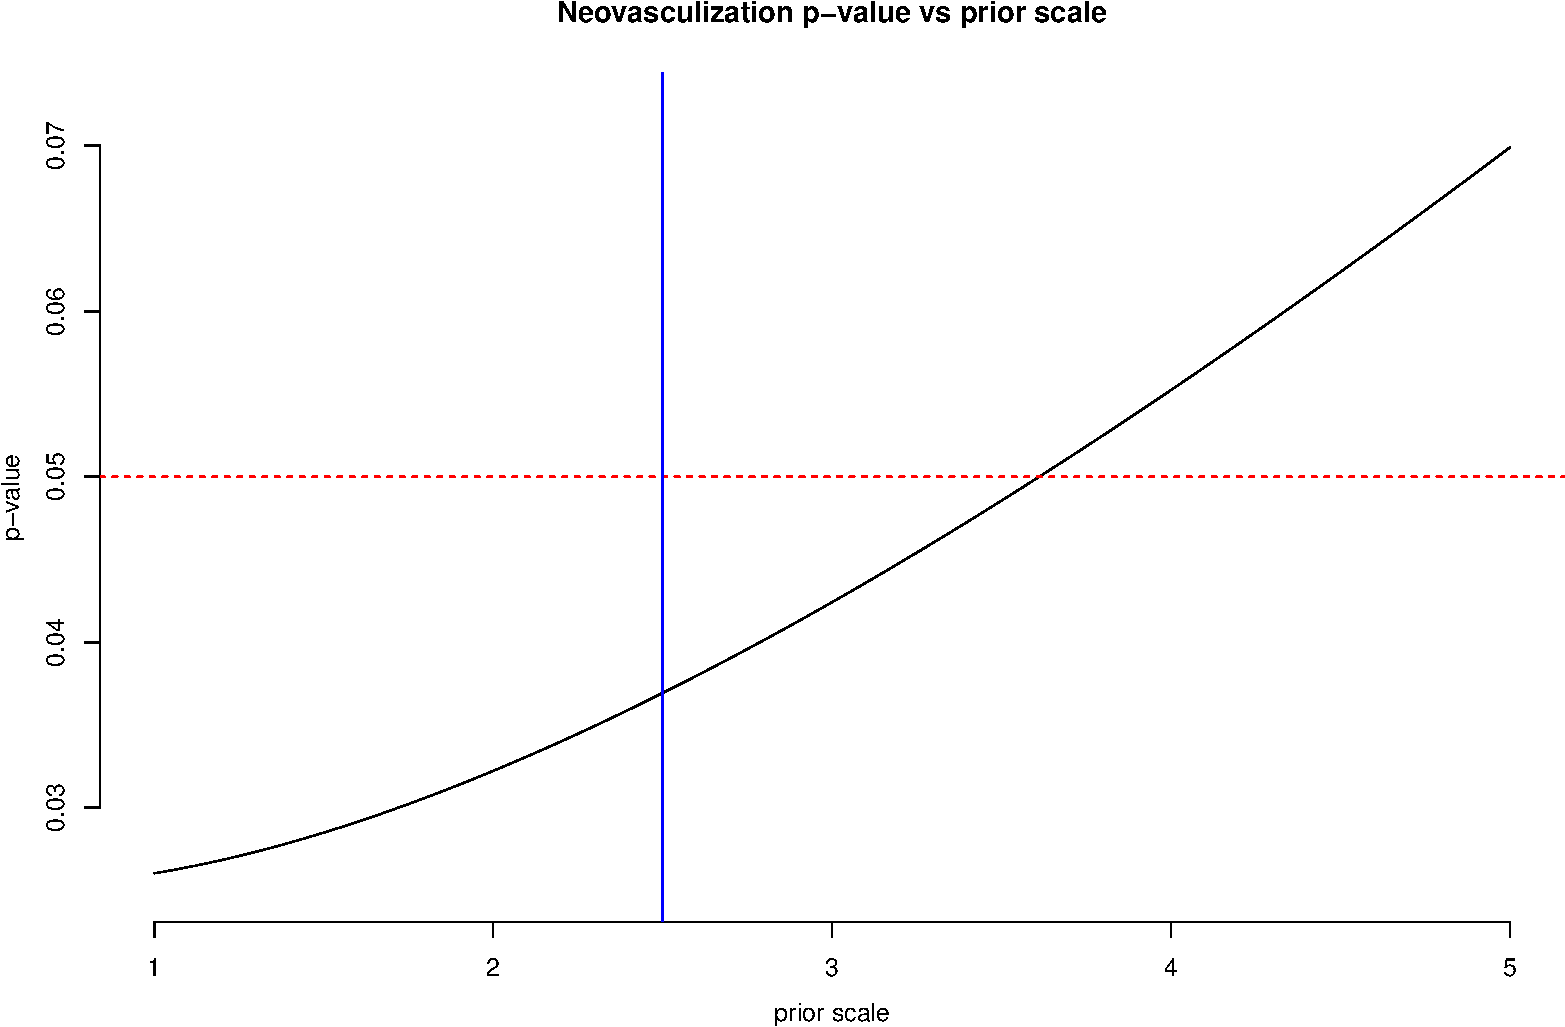
\includegraphics{week7_p2_files/figure-beamer/plot-1.pdf}
\end{frame}

\begin{frame}[fragile]{}
\protect\hypertarget{section-31}{}
Different \texttt{brglm} fitting options yield different results,
although these differences do not materialize in different conclusions
for the \texttt{NV} variable when testing at the 0.05 significance
level.

\vspace{12pt}
\tiny

\begin{Shaded}
\begin{Highlighting}[]
\FunctionTok{library}\NormalTok{(brglm2) }\CommentTok{\# for brglm2}
\NormalTok{brglm\_mod }\OtherTok{\textless{}{-}} \FunctionTok{glm}\NormalTok{(HG}\SpecialCharTok{\textasciitilde{}}\NormalTok{.,}\AttributeTok{data=}\NormalTok{endometrial,}\AttributeTok{family =} \StringTok{"binomial"}\NormalTok{,}
                 \AttributeTok{method =} \StringTok{"brglm\_fit"}\NormalTok{, }\AttributeTok{type =} \StringTok{"MPL\_Jeffreys"}\NormalTok{)}
\NormalTok{brglm\_mod\_AS\_mean }\OtherTok{\textless{}{-}} \FunctionTok{glm}\NormalTok{(HG}\SpecialCharTok{\textasciitilde{}}\NormalTok{.,}\AttributeTok{data=}\NormalTok{endometrial,}\AttributeTok{family =} \StringTok{"binomial"}\NormalTok{,}
                 \AttributeTok{method =} \StringTok{"brglm\_fit"}\NormalTok{, }\AttributeTok{type =} \StringTok{"AS\_mean"}\NormalTok{)}
\NormalTok{brglm\_mod\_AS\_median }\OtherTok{\textless{}{-}} \FunctionTok{glm}\NormalTok{(HG}\SpecialCharTok{\textasciitilde{}}\NormalTok{.,}\AttributeTok{data=}\NormalTok{endometrial,}\AttributeTok{family =} \StringTok{"binomial"}\NormalTok{,}
                         \AttributeTok{method =} \StringTok{"brglm\_fit"}\NormalTok{, }\AttributeTok{type =} \StringTok{"AS\_median"}\NormalTok{)}
\NormalTok{brglm\_mod\_AS\_mixed }\OtherTok{\textless{}{-}} \FunctionTok{glm}\NormalTok{(HG}\SpecialCharTok{\textasciitilde{}}\NormalTok{.,}\AttributeTok{data=}\NormalTok{endometrial,}\AttributeTok{family =} \StringTok{"binomial"}\NormalTok{,}
                           \AttributeTok{method =} \StringTok{"brglm\_fit"}\NormalTok{, }\AttributeTok{type =} \StringTok{"AS\_mixed"}\NormalTok{)}

\FunctionTok{c}\NormalTok{(}\FunctionTok{summary}\NormalTok{(brglm\_mod)}\SpecialCharTok{$}\NormalTok{coef[}\DecValTok{2}\NormalTok{,}\DecValTok{4}\NormalTok{], }\FunctionTok{summary}\NormalTok{(brglm\_mod\_AS\_mean)}\SpecialCharTok{$}\NormalTok{coef[}\DecValTok{2}\NormalTok{,}\DecValTok{4}\NormalTok{], }
  \FunctionTok{summary}\NormalTok{(brglm\_mod\_AS\_median)}\SpecialCharTok{$}\NormalTok{coef[}\DecValTok{2}\NormalTok{,}\DecValTok{4}\NormalTok{], }\FunctionTok{summary}\NormalTok{(brglm\_mod\_AS\_mixed)}\SpecialCharTok{$}\NormalTok{coef[}\DecValTok{2}\NormalTok{,}\DecValTok{4}\NormalTok{])}
\end{Highlighting}
\end{Shaded}

\begin{verbatim}
## [1] 0.05890214 0.05890214 0.09226858 0.05890214
\end{verbatim}
\end{frame}

\begin{frame}{Discussion}
\protect\hypertarget{discussion}{}
Which prior do we use?

\vspace{12pt}

\begin{itemize}
\tightlist
\item
  \textbf{Gelman}: Our prior {[}Cauchy \(\mu =0\); \(\sigma = 2.5\){]}
  has the advantage of always giving answers, even when there is
  complete separation in logistic regression (a common problem, even
  when the sample size is large and the number of predictors is small),
  and also automatically applying more shrinkage to higher-order
  interactions.
\item
  \textbf{Kosmidis and Firth}: Penalization of the likelihood by
  Jeffreys' invariant prior, or a positive power thereof, is shown to
  produce finite-valued maximum penalized likelihood estimates in a
  broad class of binomial generalized linear models. The class of models
  includes logistic regression, where the Jeffreys-prior penalty is
  known additionally to reduce the asymptotic bias of the maximum
  likelihood estimator
\end{itemize}
\end{frame}

\begin{frame}{}
\protect\hypertarget{section-32}{}
\begin{itemize}
\tightlist
\item
  \textbf{Gelman}: Our approach is similar {[}to Jeffrey's{]} but is
  parameterized in terms of the coefficients and thus allows us to make
  use of prior knowledge on that scale\ldots{} We recommend this prior
  distribution as a default choice for routine applied use.
\item
  \textbf{Kosmidis and Firth}: The apparent finiteness and shrinkage
  properties of the reduced-bias estimator, together with the fact that
  the estimator has the same first-order asymptotic distribution as the
  maximum likelihood estimator, are key reasons for the increasingly
  widespread use of Jeffreys-prior penalized logistic regression in
  applied work.
\item
  \textbf{Gelman}: Scale-free prior distributions such as Jeffreys' do
  not include enough prior information. As we have seen in specific
  examples and also in the corpus of datasets, this weakly-informative
  prior distribution yields estimates that make more sense and perform
  better predictively, compared to maximum likelihood.
\end{itemize}

\vspace{12pt}

\href{https://www.youtube.com/watch?v=V2f-MZ2HRHQ}{What we have here is
a failure to communicate}.
\end{frame}

\end{document}
